\chapter{GRID DETAILS}
\label{chap:grid_details}

The width of the spatial grid cells in each dimension are
\begin{align*}
  dx &= \frac{x_{\max}-x_{\min}}{n_x}, \\
  dy &= \frac{y_{\max}-y_{\min}}{n_y}, \\
  dz &= \frac{z_{\max}-z_{\min}}{n_z}.
\end{align*}
and the cell centers as
\begin{align*}
  x_i &= (i-1/2)dx \mbox{ for } i=1,\ldots,n_x, \\
  y_j &= (j-1/2)dy \mbox{ for } j=1,\ldots,n_y, \\
  z_k &= (k-1/2)dz \mbox{ for } k=1,\ldots,n_z.
\end{align*}
Denote the edges as
\begin{align*}
  x_i^e &= (i-1)dx \mbox{ for } i=1,\ldots,n_x, \\
  y_j^e &= (j-1)dy \mbox{ for } j=1,\ldots,n_y, \\
  z_k^e &= (k-1)dz \mbox{ for } k=1,\ldots,n_z.
\end{align*}

Note that in this convention, there are the same number of edges and cells,
and edges precede centers.

Now, we define the azimuthal angle such that
\begin{align*}
  \theta_l = (l-1)d\theta.
\end{align*}
For the sake of periodicity, we need
\begin{align*}
  \theta_1 &= 0, \\
  \theta_{n_\theta} &= 2\pi-d\theta,
\end{align*}
which requires
\begin{equation*}
  d\theta = \frac{2\pi}{n_\theta}.
\end{equation*}

For the polar angle, we similarly let
\begin{equation*}
  \phi_m = (m-1)d\phi.
\end{equation*}

Since the polar azimuthal is not periodic, we also store the endpoint, so
\begin{align*}
  \phi_1 &= 0, \\
  \phi_{n_\phi} &= \pi.
\end{align*}

This gives us
\begin{align*}
  d\phi &= \frac{\pi}{n_\phi-1}.
\end{align*}

It is also useful to define the edges between angular grid cells as
\begin{alignat}{3}
  \theta_l^e &= (l-1/2) d\theta, &\quad l&=1,\ldots,n_\theta \\
  \phi_m^e &= (m-1/2) d\phi, &\quad m&=1,\ldots,n_\phi-1.
\end{alignat}

Note that while $\theta$ has its final edge following its final center, this is
not the case for $\phi$, as seen in Figure \ref{fig:angular_grid_plots}.

\begin{figure}[h]
  \centering
  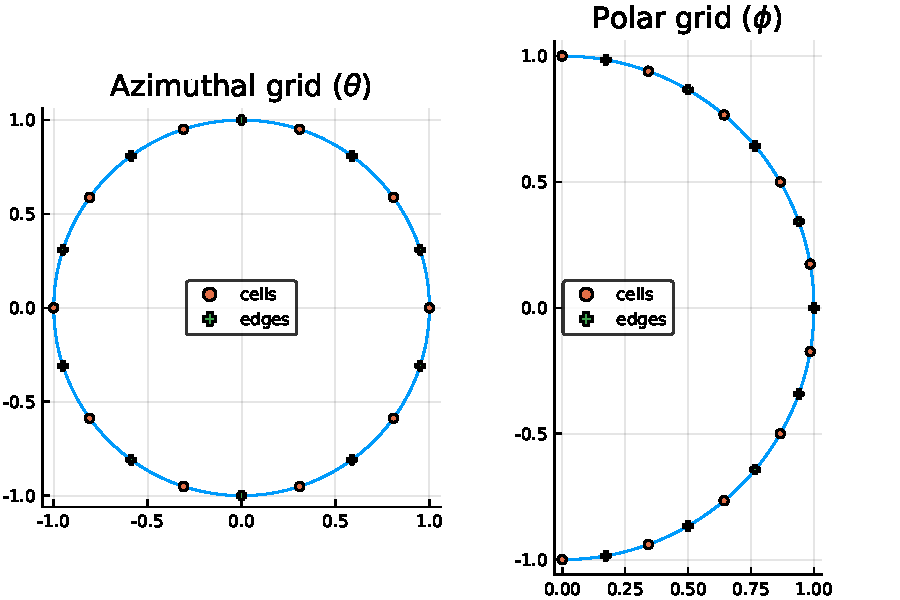
\includegraphics[width=.75\linewidth]{angular_grid_plots}
  \caption{Angular grid}
  \label{fig:angular_grid_plots}
\end{figure}

Because angles are indexed by a single integer $p$, there is a one-to-one relationship between
an integer $p$ and a pair $(l,m)$.
The relationships are as follows:
\begin{align*}
  \hat{l}(p) &= \mbox{mod1}(p, n_\theta), \\
  \hat{m}(p) &= \ceil(p/n_\theta) + 1, \\
  p &= \left( \hat{m}(p)-2\right)n_\theta + \hat{l}(p).
\end{align*}
Accordingly, define
\begin{align*}
  \hat{\theta}_p &= \theta_{\hat{l}(p)}, \\
  \hat{\phi}_p &= \phi_{\hat{m}(p)}, \\
  \hat{p}(l,m) &= (m-1)n_\theta + l.
\end{align*}

We refer to the angular grid cell centered at $\vec{\omega}_p$ as $\Omega_p$, and the solid angle subtended by $\Omega_p$ is denoted $\abs{\Omega_p}$.
The areas of the grid cells are calculated as follows.
Note that there is a temporary abuse of notation in that the same symbols ($d\theta$ and $d\phi$) are being used for infinitesimal differential and for finite grid spacing.
For the poles, we have
\begin{align*}
  \abs{\Omega_1} = \abs{\Omega_\nomega} &= \int_{\Omega_1} d{\vec{\omega}} \\
  &= \int_0^{2\pi}\int_0^{d\phi/2} \sin\phi\, d\phi\, d\theta \\
  &= 2\pi \cos\phi \Big|_{d\phi/2}^0 \\
  &= 2\pi(1-\cos(d\phi/2)).
\end{align*}
For all other angular grid cells,
\begin{align*}
  \abs{\Omega_p} &= \int_{\Omega_p} d{\vec{\omega}} \\
                 &= \int_{\theta_l^e}^{\theta_{l+1}^e}\int_{\phi_m^e}^{\phi_{m+1}^e} \sin(\phi)\, d\phi\, d\theta \\
                 &= d\theta \int_{\phi_m^e}^{\phi_{m+1}^e} \sin(\phi)\, d\phi \\
                 &= d\theta\left( \cos(\phi_m^e)-\cos(\phi_{m+1}^e) \right).
\end{align*}
